\documentclass[tikz,border=8pt]{standalone}
\usepackage{tikz}
\usetikzlibrary{arrows.meta, positioning, fit, shapes.geometric}

\begin{document}
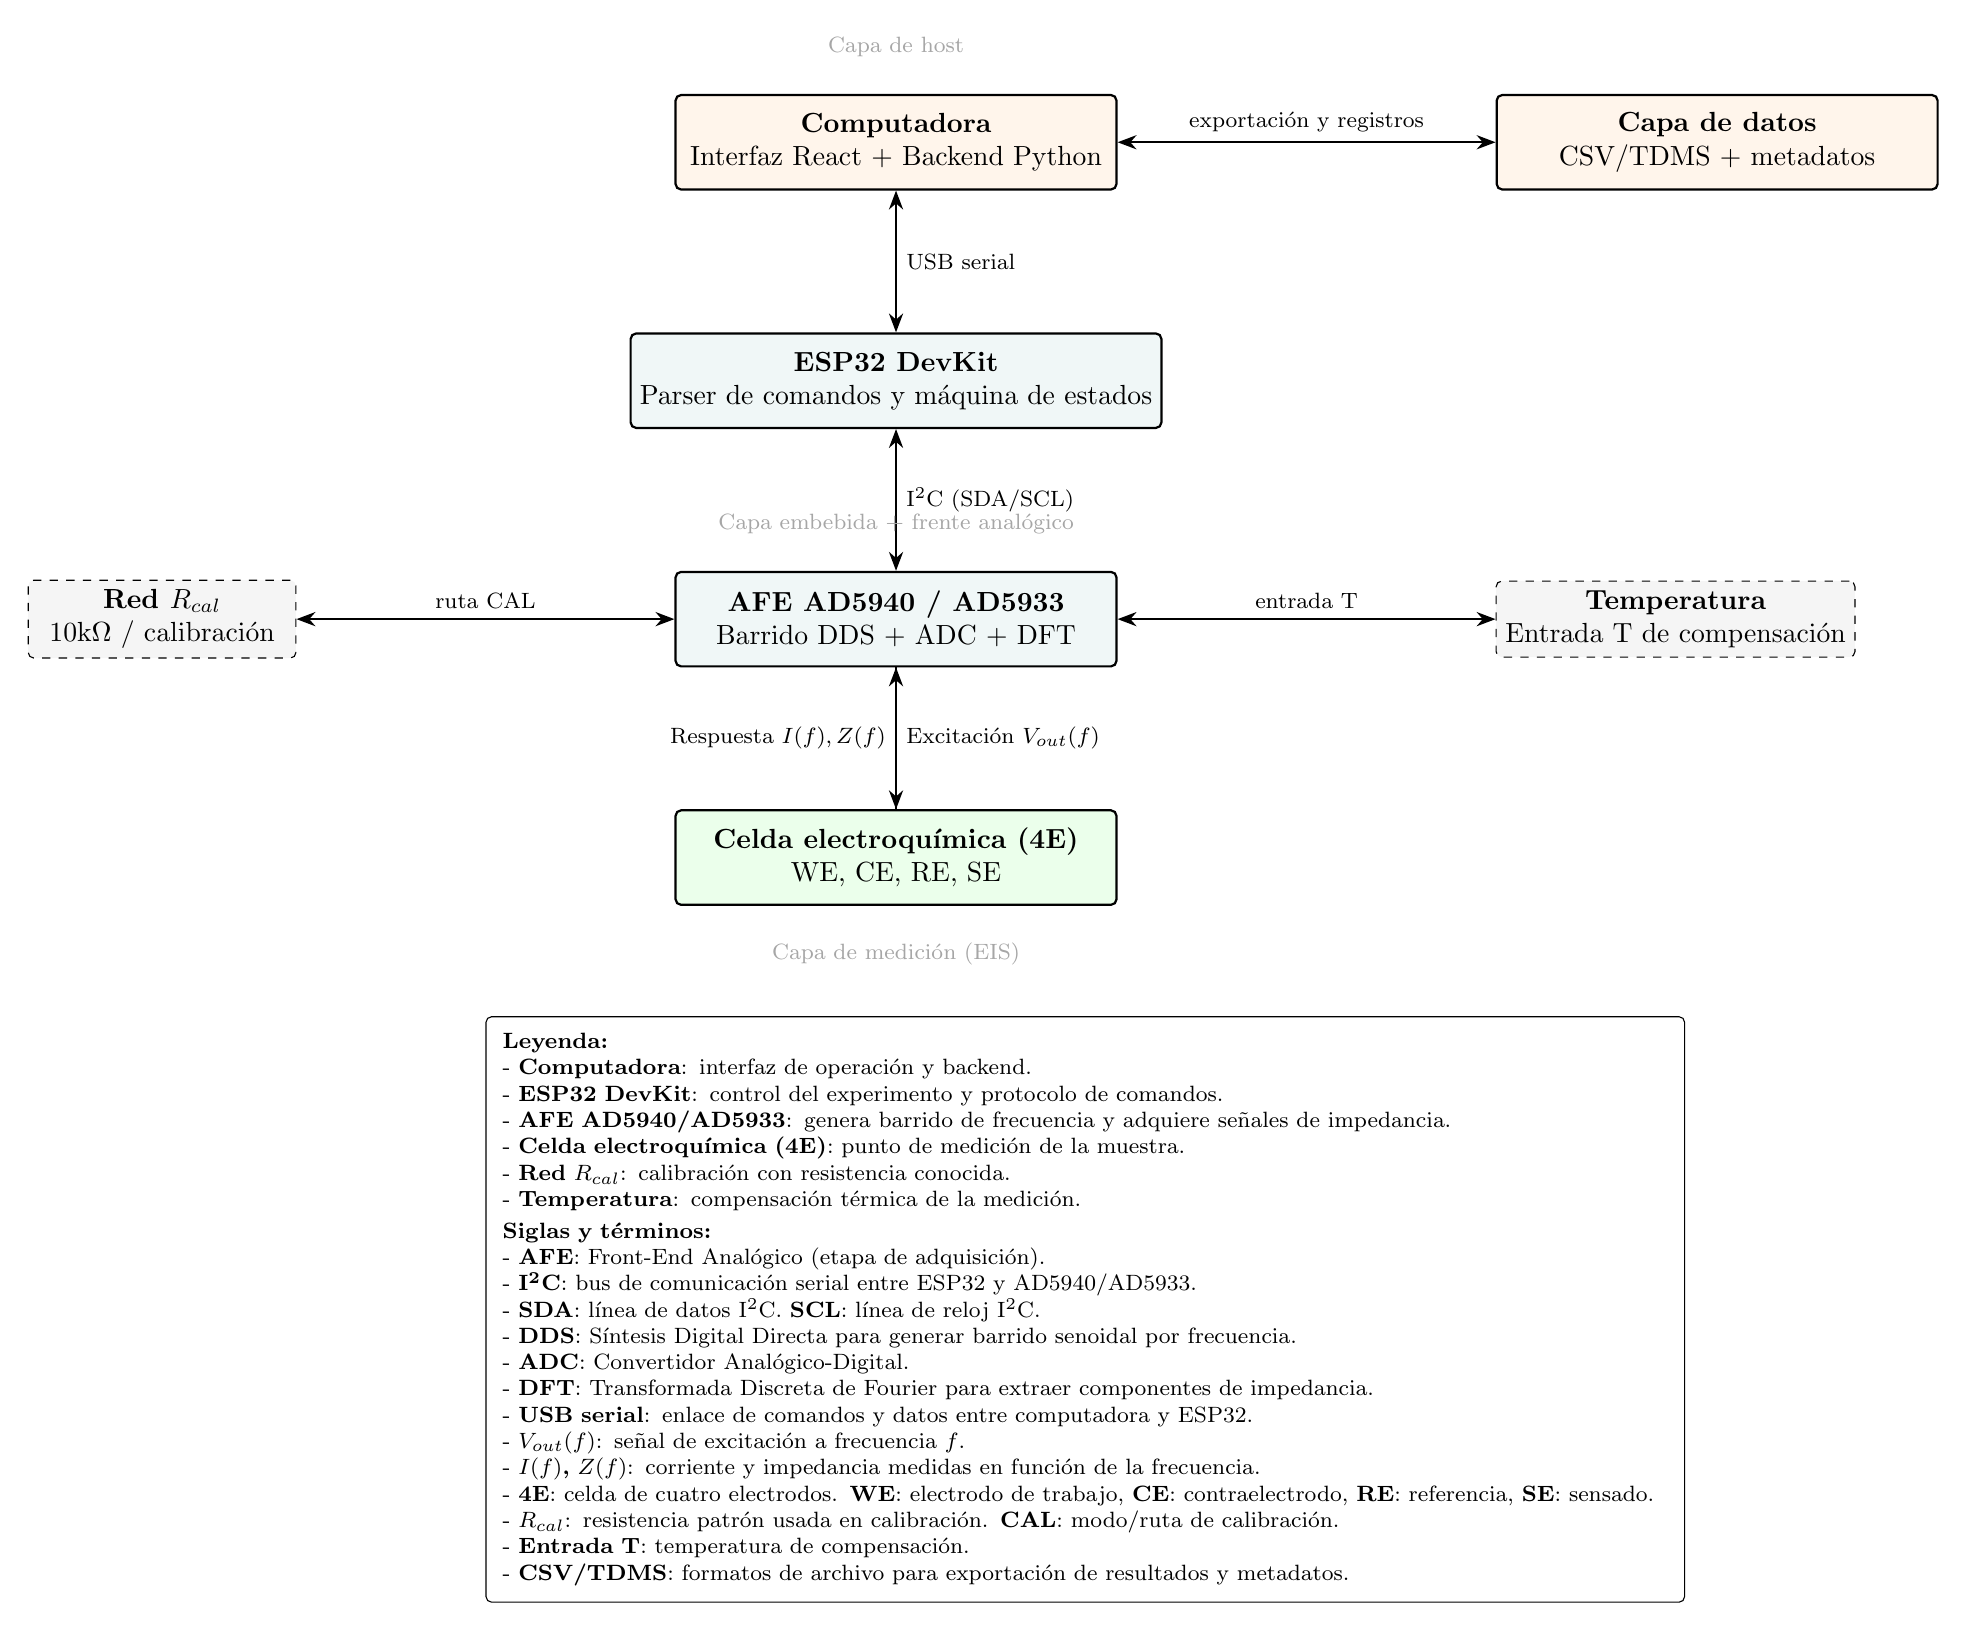
\begin{tikzpicture}[
  block/.style={draw, rounded corners=2pt, thick, align=center, minimum height=1.2cm, minimum width=5.6cm, fill=blue!4},
  hw/.style={block, fill=teal!6},
  sw/.style={block, fill=orange!8},
  elec/.style={block, fill=green!8},
  aux/.style={draw, dashed, rounded corners=2pt, align=center, minimum height=0.9cm, minimum width=3.4cm, fill=gray!8},
  line/.style={thick, -{Stealth[length=2.4mm]}},
  bline/.style={thick, {Stealth[length=2.4mm]}-{Stealth[length=2.4mm]}},
  note/.style={font=\footnotesize, text=gray!70}
]

% Eje principal vertical
\node[sw] (pc) at (0,0) {\textbf{Computadora}\\Interfaz React + Backend Python};
\node[hw, below=1.8cm of pc] (esp) {\textbf{ESP32 DevKit}\\Parser de comandos y m\'aquina de estados};
\node[hw, below=1.8cm of esp] (afe) {\textbf{AFE AD5940 / AD5933}\\Barrido DDS + ADC + DFT};
\node[elec, below=1.8cm of afe] (cell) {\textbf{Celda electroqu\'imica (4E)}\\WE, CE, RE, SE};

% Bloques auxiliares laterales
\node[sw, right=4.8cm of pc] (log) {\textbf{Capa de datos}\\CSV/TDMS + metadatos};
\node[aux, right=4.8cm of afe] (temp) {\textbf{Temperatura}\\Entrada T de compensaci\'on};
\node[aux, left=4.8cm of afe] (rcal) {\textbf{Red $R_{cal}$}\\10k$\Omega$ / calibraci\'on};

% Conexiones principales
\draw[bline] (pc) -- node[right,font=\footnotesize]{USB serial} (esp);
\draw[bline] (esp) -- node[right,font=\footnotesize]{I\textsuperscript{2}C (SDA/SCL)} (afe);
\draw[line] (afe) -- node[right,font=\footnotesize]{Excitaci\'on $V_{out}(f)$} (cell);
\draw[line] (cell) -- node[left,font=\footnotesize]{Respuesta $I(f), Z(f)$} (afe);

% Conexiones laterales
\draw[bline] (pc.east) -- node[above,font=\footnotesize]{exportaci\'on y registros} (log.west);
\draw[bline] (rcal.east) -- node[above,font=\footnotesize]{ruta CAL} (afe.west);
\draw[bline] (temp.west) -- node[above,font=\footnotesize]{entrada T} (afe.east);

% Notas de capas
\node[note, above=0.35cm of pc] {Capa de host};
\node[note, above=0.35cm of afe] {Capa embebida + frente anal\'ogico};
\node[note, below=0.35cm of cell] {Capa de medici\'on (EIS)};

% Leyenda inferior (lista vertical, alineada a la izquierda)
\node[draw, rounded corners=2pt, align=left, fill=white, font=\footnotesize,
      text width=14.8cm, inner sep=6pt, anchor=north west]
      (legend) at ([xshift=-2.4cm,yshift=-1.4cm]cell.south west) {
\textbf{Leyenda:}\\
- \textbf{Computadora}: interfaz de operaci\'on y backend.\\
- \textbf{ESP32 DevKit}: control del experimento y protocolo de comandos.\\
- \textbf{AFE AD5940/AD5933}: genera barrido de frecuencia y adquiere se\~nales de impedancia.\\
- \textbf{Celda electroqu\'imica (4E)}: punto de medici\'on de la muestra.\\
- \textbf{Red $R_{cal}$}: calibraci\'on con resistencia conocida.\\
- \textbf{Temperatura}: compensaci\'on t\'ermica de la medici\'on.\\[2pt]
\textbf{Siglas y t\'erminos:}\\
- \textbf{AFE}: Front-End Anal\'ogico (etapa de adquisici\'on).\\
- \textbf{I\textsuperscript{2}C}: bus de comunicaci\'on serial entre ESP32 y AD5940/AD5933.\\
- \textbf{SDA}: l\'inea de datos I\textsuperscript{2}C. \textbf{SCL}: l\'inea de reloj I\textsuperscript{2}C.\\
- \textbf{DDS}: S\'intesis Digital Directa para generar barrido senoidal por frecuencia.\\
- \textbf{ADC}: Convertidor Anal\'ogico-Digital.\\
- \textbf{DFT}: Transformada Discreta de Fourier para extraer componentes de impedancia.\\
- \textbf{USB serial}: enlace de comandos y datos entre computadora y ESP32.\\
- \textbf{$V_{out}(f)$}: se\~nal de excitaci\'on a frecuencia $f$.\\
- \textbf{$I(f)$, $Z(f)$}: corriente y impedancia medidas en funci\'on de la frecuencia.\\
- \textbf{4E}: celda de cuatro electrodos. \textbf{WE}: electrodo de trabajo, \textbf{CE}: contraelectrodo, \textbf{RE}: referencia, \textbf{SE}: sensado.\\
- \textbf{$R_{cal}$}: resistencia patr\'on usada en calibraci\'on. \textbf{CAL}: modo/ruta de calibraci\'on.\\
- \textbf{Entrada T}: temperatura de compensaci\'on.\\
- \textbf{CSV/TDMS}: formatos de archivo para exportaci\'on de resultados y metadatos.
};

\end{tikzpicture}
\end{document}
